% SC3270 --- Chapter 5: Termination - Proving Programs Stop (0->100 ground-up)
\chapter{Termination: Proving Programs Stop}
\label{ch:termination}

\begin{quote}
\emph{``A program that never stops is correct in the most useless sense: it never gives a wrong answer because it never gives any answer.''} We now prove that loops actually finish.
\end{quote}

\noindent\fbox{\parbox{\dimexpr\linewidth-2\fboxsep-2\fboxrule}{%
\textbf{From zero: no termination theory assumed.} We define partial vs.\ total correctness, introduce variants (ranking functions) and well-founded orders, and prove termination of standard loops. Lexicographic orders and non-termination counterexamples follow.}}
\vspace{0.4em}

\section*{Learning Outcomes}
After this chapter you will be able to:
\begin{enumerate}[label=(L\arabic*)]
    \item distinguish partial and total correctness and state what total adds;
    \item define variant and well-founded order and explain why they force termination;
    \item prove termination of single and nested loops via numeric and lexicographic variants;
    \item exhibit a loop that fails to terminate and diagnose why no variant exists;
    \item state the total-correctness while-rule and apply it end-to-end.
\end{enumerate}

% ============================================================
\section{Partial Is Not Enough}
\label{sec:partial-not-enough}
\paragraph{Intuition.} Recall $\{P\}\,C\,\{Q\}$ means ``if $C$ terminates from $P$, then $Q$.'' A loop that never terminates satisfies \emph{every} partial triple—vacuously. The canonical villain:
\[
\{\text{true}\}\;\texttt{while true do skip}\;\{\text{false}\}
\]
is partially correct (no terminating execution to refute $\text{false}$) yet clearly wrong in practice. Total correctness $[P]\,C\,[Q]$ strengthens the promise: ``$C$ \emph{does} terminate from $P$ and then $Q$ holds.'' So total $=$ partial $+$ termination.

\begin{figure}[h]\centering
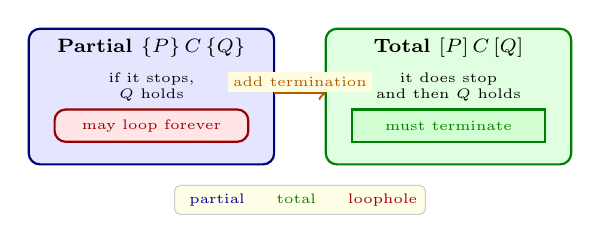
\begin{tikzpicture}[scale=0.82,font=\scriptsize]
\draw[fill=blue!10,draw=blue!50!black,thick,rounded corners=4pt] (0,0) rectangle (3.8,2.1);
\node at (1.9,1.80) {\textbf{Partial $\{P\}\,C\,\{Q\}$}};
\node[font=\tiny,align=center] at (1.9,1.20) {if it stops,\\ $Q$ holds};
\draw[fill=red!10,draw=red!60!black,thick,rounded corners=4pt] (0.4,0.35) rectangle (3.4,0.85);
\node[font=\tiny,red!60!black] at (1.9,0.60) {may loop forever};
\draw[fill=green!12,draw=green!50!black,thick,rounded corners=4pt] (4.6,0) rectangle (8.4,2.1);
\node at (6.50,1.80) {\textbf{Total $[P]\,C\,[Q]$}};
\node[font=\tiny,align=center] at (6.50,1.20) {it does stop\\ and then $Q$ holds};
\draw[fill=green!18,draw=green!50!black,thick] (5.0,0.35) rectangle (8.0,0.85);
\node[font=\tiny,green!50!black] at (6.50,0.60) {must terminate};
\draw[->,thick,orange!70!black] (3.8,1.10) -- (4.6,1.10) node[midway,above,font=\tiny,fill=yellow!12,inner sep=2pt] {add termination};
\node[font=\tiny,align=left,fill=yellow!10,draw=gray!40,rounded corners=2pt,inner sep=3pt] at (4.2,-0.55) {\textcolor{blue!60!black}{$\blacksquare$ partial} \quad \textcolor{green!50!black}{$\blacksquare$ total} \quad \textcolor{red!60!black}{$\blacksquare$ loophole}};
\end{tikzpicture}
\caption{Partial correctness allows infinite executions (red strip); total correctness forbids them. Termination is the missing conjunct.}
\label{fig:partial-vs-total}
\end{figure}

\begin{definition}[Partial vs total]
$\{P\}\,C\,\{Q\}$ is \emph{partial}: $\forall\sigma\in\llbracket P\rrbracket.\; C(\sigma)\downarrow \sigma' \Rightarrow \sigma'\in\llbracket Q\rrbracket$. $[P]\,C\,[Q]$ is \emph{total}: $\forall\sigma\in\llbracket P\rrbracket.\; C(\sigma)\downarrow \sigma' \land \sigma'\in\llbracket Q\rrbracket$, where $\downarrow$ means terminates. For loop-free $C$, the two coincide.
\end{definition}

% ============================================================
\section{Variants: Numbers That Must Hit Zero}
\label{sec:variants}
\paragraph{Intuition.} Imagine stairs labelled $5,4,3,2,1,0$. You start at some step and promise to go down by at least one each lap, never below $0$. You must hit $0$ within $5$ laps. A \emph{variant} (ranking function) $V:\text{State}\to\mathbb{N}$ is that stair number: a natural that strictly decreases each iteration and is bounded below by $0$. No infinite descent in $\mathbb{N}$ exists, so the loop cannot loop forever.

\begin{definition}[Variant and well-founded]
A \emph{variant} for \texttt{while $B$ do $C$} with invariant $I$ is an expression $V$ such that (i) $I\land B \Rightarrow V\ge0$, and (ii) $\{I\land B\land V=v_0\}\,C\,\{V<v_0\}$ where $v_0$ is a fresh logical variable capturing the entry value. More generally $V$ maps to any \emph{well-founded} order (no infinite descending chains), e.g.\ lexicographic pairs.
\end{definition}

\begin{figure}[h]\centering
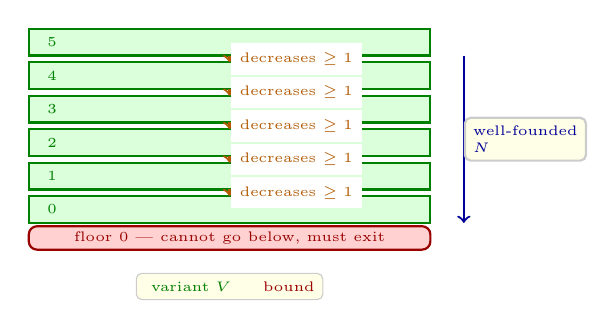
\begin{tikzpicture}[scale=0.85,font=\scriptsize]
\foreach \y/\lab in {2.8/5,2.3/4,1.8/3,1.3/2,0.8/1,0.3/0} {
  \draw[fill=green!14,draw=green!50!black,thick] (0.5,\y) rectangle (6.5,\y+0.40);
  \node[font=\tiny,green!50!black] at (0.85,\y+0.20) {\lab};
}
\foreach \y in {2.8,2.3,1.8,1.3,0.8} \draw[->,thick,orange!70!black] (3.5,\y) -- (3.5,\y-0.10) node[midway,right,font=\tiny,fill=white] {decreases $\ge1$};
\draw[fill=red!18,draw=red!60!black,thick,rounded corners=3pt] (0.5,-0.10) rectangle (6.5,0.25);
\node[font=\tiny,red!60!black] at (3.5,0.08) {floor $0$ --- cannot go below, must exit};
\draw[->,thick,blue!60!black] (7.0,2.8) -- (7.0,0.3) node[midway,right,font=\tiny,align=left,fill=yellow!10,draw=gray!40,rounded corners=2pt,inner sep=3pt] {well-founded\\ $\mathbb{N}$};
\node[font=\tiny,align=left,fill=yellow!10,draw=gray!40,rounded corners=2pt,inner sep=3pt] at (3.5,-0.65) {\textcolor{green!50!black}{$\blacksquare$ variant $V$} \quad \textcolor{red!60!black}{$\blacksquare$ bound}};
\end{tikzpicture}
\caption{Variant as staircase: $V$ starts at some $n\ge0$ and drops by at least one each iteration. Hitting $0$ is inevitable; infinite looping would require infinite descent in $\mathbb{N}$, which is impossible.}
\label{fig:variant-staircase}
\end{figure}

\begin{figure}[h]\centering
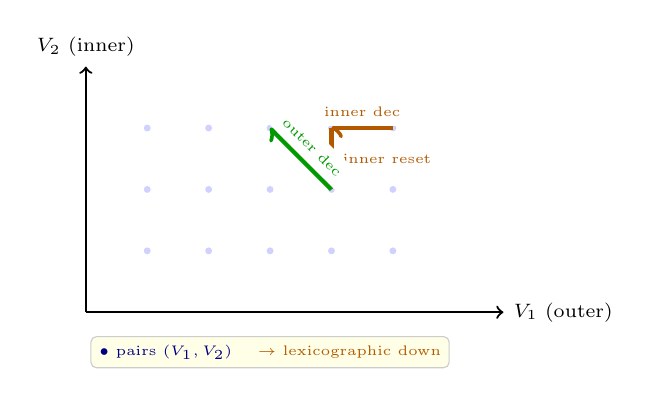
\begin{tikzpicture}[scale=0.78,font=\scriptsize]
\draw[->,thick] (0,0) -- (6.8,0) node[right] {$V_1$ (outer)};
\draw[->,thick] (0,0) -- (0,4.0) node[above] {$V_2$ (inner)};
\foreach \x in {1,2,3,4,5} \foreach \y in {1,2,3} \fill[blue!18] (\x,\y) circle (1.6pt);
\draw[->,ultra thick,orange!70!black] (5,3) -- (4,3) node[midway,above,font=\tiny,fill=white] {inner dec};
\draw[->,ultra thick,orange!70!black] (4,3) -- (4,2) node[midway,right,font=\tiny,fill=white] {inner reset};
\draw[->,ultra thick,green!60!black] (4,2) -- (3,3) node[midway,above,sloped,font=\tiny,fill=white] {outer dec};
\node[font=\tiny,align=left,fill=yellow!10,draw=gray!40,rounded corners=2pt,inner sep=3pt] at (3.0,-0.65) {\textcolor{blue!50!black}{$\bullet$ pairs $(V_1,V_2)$} \quad \textcolor{orange!70!black}{$\to$ lexicographic down}};
\end{tikzpicture}
\caption{Lexicographic order $(V_1,V_2)$: compare $V_1$ first, then $V_2$. Inner loop decreases $V_2$ while $V_1$ stays; outer decreases $V_1$ and resets $V_2$. Any lexicographic descent in $\mathbb{N}\times\mathbb{N}$ is finite.}
\label{fig:lexicographic}
\end{figure}

% ============================================================
\section{Proving Total Correctness}
\label{sec:proving-total}
Total while-rule (one form):
\[
\frac{\{I\land B\land V=v_0\}\,C\,\{I\land V<v_0\}\qquad I\land B\Rightarrow V\ge0}{\{I\}\,\texttt{while }B\texttt{ do }C\,\{I\land\neg B\}}\ \text{(total)}.
\]
Together with $P\Rightarrow I$ and $I\land\neg B\Rightarrow Q$ this gives $[P]\,\texttt{while }B\texttt{ do }C\,[Q]$.

\begin{example}[Countdown]
$[n\ge0]\;x:=n;\;\texttt{while }x>0\texttt{ do }x:=x-1\;[x=0]$ with $I\equiv0\le x\le n$ and variant $V\equiv x$. Check: $I\land x>0\Rightarrow x\ge1\Rightarrow V\ge0$, and $\{x=v_0\}\,x:=x-1\,\{x=v_0-1 < v_0\}$. So variant drops by one; termination in $n$ steps.
\end{example}

\begin{example}[Nested loops]
Outer $i:=0;\texttt{while }i<n\texttt{ do }(j:=0;\texttt{while }j<m\texttt{ do }j:=j+1;\,i:=i+1)$ has lexicographic variant $(n-i,\; m-j)$ ordered lexicographically: inner decreases second component, outer decreases first and resets second to $m$. No infinite lexicographic descent exists.
\end{example}

\begin{example}[Euclid total]
Euclid loop $I\equiv a>0\land b>0\land\gcd(a,b)=\gcd(a_0,b_0)$, $V\equiv a+b$. Each iteration replaces $(a,b)$ with $(a-b,b)$ or $(a,b-a)$, so $V$ drops by $\min(a,b)\ge1$ and stays $\ge2$. Hence Euclid terminates and then $a=b=\gcd(a_0,b_0)$—total correctness in one invariant plus one variant.
\end{example}

\begin{lstlisting}[language=Python, caption={Variant as runtime monitor: assert decrease and boundedness each lap.}, label={lst:variant-py}]
def countdown(n):
    x = n
    # I: 0<=x<=n, variant V=x
    assert 0 <= x <= n
    while x > 0:
        v0 = x
        assert x >= 0          # bounded
        x -= 1
        assert x < v0          # decreased
        assert 0 <= x <= n     # invariant preserved
    assert x == 0
\end{lstlisting}

% ============================================================
\section{When Termination Fails}
\label{sec:nonterm}
Loop \texttt{while $x\neq0$ do } \texttt{if $x>0$ then $x:=x-1$ else $x:=x+1$} with $I\equiv\text{true}$ and would-be variant $|x|$ does \emph{not} decrease when $x<0$? Actually it does ($|{-2}|=2\to|{-1}|=1$). Try instead \texttt{while $x>0$ do $x:=x+1$}: variant $x$ \emph{increases}, and no $V\ge0$ that decreases exists—the loop diverges for $x>0$. Diagnosis: cannot find $V$ with $I\land B\Rightarrow V\ge0$ and strict decrease; the attempt to synthesize $V$ fails, revealing the bug.

Halting in general is undecidable (Turing), so no uniform variant synthesis can succeed for all programs. For restricted loops (affine guards and updates) synthesis is decidable—this is active verification research.

\begin{lstlisting}[language=C, caption={A terminating and a non-terminating loop: only one admits a variant.}, label={lst:term-c}]
// Terminates: variant n-x decreases
int x=0; while(x < n){ x++; } // V = n - x

// Diverges when n>0: no variant decreases
int y=1; while(y != 0){ y = y+1; } // overflows? unbounded increase
\end{lstlisting}

% ============================================================
\section{\texorpdfstring{Well-Founded Orders Beyond $\mathbb{N}$}{Well-Founded Orders Beyond N}}
\label{sec:wf-beyond}
$\mathbb{N}$ suffices for many loops, but some need richer orders. Consider traversing a binary tree with a worklist: variant is multiset of remaining node heights, ordered by multiset extension of $<$—still well-founded. Another is Ackermann's function: variant is the pair $(m,n)$ with lexicographic order on $\mathbb{N}\times\mathbb{N}$, which decreases in each recursive call even though a single number does not.

Key property: a relation $\prec$ is \emph{well-founded} if every non-empty set has a minimal element, equivalently no infinite descending chain $x_0\succ x_1\succ\cdots$ exists. $\mathbb{N}$ with $<$ is well-founded; $\mathbb{Z}$ with $<$ is not (go to $-\infty$ forever); $\mathbb{N}\times\mathbb{N}$ lexicographically is well-founded (Dickson's lemma intuition). Choosing the right order is the creative step when a plain integer variant fails.

\begin{example}[Ackermann variant]
Ackermann $A(m,n)$ recursion: if $m=0$ then $n+1$ else if $n=0$ then $A(m-1,1)$ else $A(m-1,A(m,n-1))$. Each call reduces $(m,n)$ lexicographically: either $m$ drops, or $m$ stays and $n$ drops. Lexicographic well-foundedness guarantees termination despite the nested recursion that defeats a simple $m+n$ variant.
\end{example}

\begin{remark}[Why $\mathbb{N}$ and not $\mathbb{Z}$?]
$\mathbb{Z}$ is not well-founded because $\cdots 3>2>1>0>-1>-2>\cdots$ is infinite descent. So $V:\text{State}\to\mathbb{Z}$ with only $V\ge0$ as lower bound would not guarantee termination—you could stay $\ge0$ forever while descending $100,99,98,\dots$? Actually that still terminates at $0$; the danger is you could descend $0,-1,-2,\dots$ and never hit the bound. Requiring $V\ge0$ \emph{and} mapped to $\mathbb{N}$ excludes negative descent.
\end{remark}

\begin{remark}[Invariant vs variant]
Invariant answers ``what stays true''; variant answers ``what gets smaller''. Invariant is checked once per lap (holds before and after); variant is compared across the lap ($V_{\text{after}}<V_{\text{before}}$). A loop needs both: invariant for correctness when it stops, variant to guarantee it does stop. One without the other is half a proof.
\end{remark}

% ============================================================
\section{Connecting to Decidability}
\label{sec:decidability}
Turing proved halting is undecidable: no program can decide termination for all programs. So variant synthesis cannot be fully automatic. Yet for many practical loops—affine guards $a\cdot x + b > 0$ and linear updates—synthesis is decidable via linear ranking functions (Podelski--Rybalchenko). Modern verifiers try linear templates $V = c_0 + \sum c_i x_i$ and solve for $c_i$ that satisfy the two variant conditions via linear programming. When they succeed, you get termination for free; when they fail, you must supply a lexicographic or non-linear variant manually. This interplay is why verification remains a human-machine collaboration.

% ============================================================
\section{Full Total-Correctness Proof: Linear Search}
\label{sec:search-total}
Claim: $[n\ge0]\; i:=0;\,\texttt{while }i<n\land a[i]\neq key\texttt{ do }i:=i+1\; [ (i=n\Rightarrow\forall j<n.\,a[j]\neq key)\land(i<n\Rightarrow a[i]=key)]$.

We already have $I\equiv 0\le i\le n\land\forall j<i.\,a[j]\neq key$ for partial. Add variant $V\equiv n-i$. Check: $I\land i<n\land a[i]\neq key\Rightarrow n-i>0\Rightarrow V\ge0$, and body $i:=i+1$ maps $V=n-i$ to $V'=n-(i+1)=V-1<V$. So total holds. Exit $I\land\neg(i<n\land a[i]\neq key)$ splits: either $i=n$ (exhausted, so $\forall j<n.\,a[j]\neq key$ from $I$) or $a[i]=key$ (found). No divergence case remains—variant forced exit within $n$ steps.

This illustrates the methodology: prove partial with $I$, then reuse $I$ and add $V$ for total. The two proofs compose; you never re-prove $I$ preservation.

% ============================================================
\section{Exercises}
\label{sec:ch05-exercises}
\begin{enumerate}[label=E5.\arabic*, leftmargin=*, itemsep=0.6em]
    \item \textbf{Countdown variant.} Prove $[n\ge0]\,x:=n;\texttt{while }x>0\texttt{ do }x:=x-1\,[x=0]$ with $I\equiv0\le x\le n$, $V\equiv x$ by checking both variant conditions.
    \item \textbf{Lexicographic.} Give lexicographic variant for double loop summing $a[m][n]$ row-major and argue why single $n-i+m-j$ also works but is less modular.
    \item \textbf{Non-termination witness.} Give $P,B,C$ where $\{P\land B\}\,C\,\{P\}$ holds (so partial proof succeeds) but no variant exists. Explain why the partial triple is vacuously useful.
    \item \textbf{Euclid variant.} For Euclid with $\gcd$, propose variant $a+b$ and prove it decreases when replacing $(a,b)$ by $(a-b,b)$ or $(a,b-a)$.
    \item \textbf{Total triple.} State total triple for linear search that guarantees it stops, and give invariant plus variant; show exit post now includes ``found or not found'' without divergence loophole.
\end{enumerate}

\section*{Chapter Notes}
Variants are Dijkstra's invention; well-founded orders come from set theory (Kunen). Lexicographic termination appears in Floyd and Manna. For undecidability see Sipser Ch.~4; for synthesis for linear loops see Podelski--Rybalchenko. Practice: after each invariant, immediately ask ``what gets smaller?'' and write $V$ next to $I$.

\smallskip
\begin{remark}[Variant discovery heuristic]
Good $V$ often mirrors the guard's distance to falsity: \texttt{while $x>0$} suggests $V=x$; \texttt{while $i<n$} suggests $V=n-i$; \texttt{while $a\neq b$} suggests $V=|a-b|$ or $a+b$. If guard is $x\neq y$, ask ``what measure of $x$ vs $y$ shrinks?'' The guard's shape hints at $V$.
\end{remark}

\smallskip
\begin{remark}[Check total early]
During code review ask ``does this loop have a variant?'' before ``is this invariant correct?'' Non-termination bugs (infinite loops on edge inputs) are often cheaper to fix than postcondition bugs, and the variant question surfaces them immediately.
\end{remark}
% End of Chapter 5
